% Informe Proyecto 2 (versión final). Compilar con pdfLaTeX (MiKTeX, Prism u Overleaf), dos pasadas: main.tex + carpeta figs/.
% Compilado: 9 páginas (el límite es 10). Si se agrega contenido, reducir el ancho de las figuras o quitar el lienzo (Sección 2).
\documentclass[11pt,letterpaper]{article}
\usepackage[utf8]{inputenc}
\usepackage[T1]{fontenc}
\usepackage{lmodern}  % fuentes vectoriales (sin esto, MiKTeX genera mapas de bits)
\usepackage[spanish,es-tabla,es-nodecimaldot,es-noshorthands]{babel}
\usepackage[margin=1in]{geometry}
\usepackage{graphicx}
\usepackage{booktabs}
\usepackage{tabularx}
\usepackage{array}
\usepackage{float}
\usepackage{xcolor}
\usepackage{titlesec}
\usepackage{enumitem}
\usepackage{caption}
\usepackage{amssymb}
\usepackage[hidelinks]{hyperref}

\definecolor{utecblue}{RGB}{18,53,91}
\titleformat{\section}{\color{utecblue}\large\bfseries}{\thesection.}{0.6em}{}
\titleformat{\subsection}{\bfseries}{\thesubsection.}{0.5em}{}
\titlespacing*{\section}{0pt}{1.4ex plus .4ex}{0.8ex}
\titlespacing*{\subsection}{0pt}{1.0ex plus .3ex}{0.4ex}
\setlist{itemsep=1pt,topsep=3pt}
\setlist[itemize]{label=\scriptsize$\blacksquare$}
\captionsetup{font=small,labelsep=colon}
\setlength{\parskip}{0.5ex}
\setlength{\parindent}{0pt}
\newcolumntype{L}{>{\raggedright\arraybackslash}X}

\begin{document}

% ------------------------------------------------------------------ portada
\begin{titlepage}
\centering
\vspace*{0.6cm}

\includegraphics[width=0.27\textwidth]{figs/logo_utec.png}\par\vspace{1.0cm}
{\Large\bfseries UNIVERSIDAD DE INGENIERÍA Y TECNOLOGÍA\par}\vspace{0.4cm}
{\large Facultad de Computación\par}\vspace{0.4cm}
{\large\bfseries Planificación y Toma de Decisiones en IA (CS5363)\par}\vspace{1.4cm}
{\LARGE\bfseries Vitrina IA: Probador Virtual de Estilos de Vestimenta para Tiendas de Moda en Línea\par}\vspace{0.4cm}
{\large Sistema generativo interactivo con feedback humano y explicación mediante agentes de IA\par}\vspace{0.5cm}
{\normalsize Proyecto 2 -- Informe final: sistema implementado, resultados y limitaciones\par}
\vspace{1.4cm}
{\bfseries Integrantes\par}\vspace{0.25cm}
Edgar Moisés Chambilla Mamani\\
Jose Joaquin Osnayo Matos\\
Luis Anthony Romero Padilla\\
Andrés Martín Benjamín Torres Ramos\\
Jose Francisco Wong Orrillo\par
\vspace{0.6cm}
{\bfseries Profesores\par}\vspace{0.25cm}
Dra. Aurea Soriano-Vargas\\
Mg. Robert Buleje-Del-Carpio\par
\vfill
{\bfseries Lima, Perú -- Noviembre de 2026\par}
\end{titlepage}
\setcounter{page}{1}

% ------------------------------------------------------------------ 1
\section{Definición del problema}

\textbf{Contexto y problema.} Comprar ropa por internet obliga a decidir sin probarse la prenda: el cliente la ve sobre
un modelo con otro cuerpo, otro tono de piel y otra pose, y debe imaginar cómo le quedaría. Esa incertidumbre frena la
compra y termina en devoluciones. ¿Cómo puede una tienda mostrar a cada cliente \textbf{cómo se vería él mismo} con
distintas prendas, a partir de una sola fotografía, sin alterar su identidad y dejando la decisión en sus manos?
Lo planteamos como \textbf{toma de decisiones asistida}: la IA propone exactamente cinco looks sobre la foto del
cliente; él acepta o rechaza cada uno; el sistema registra las decisiones y vuelve a generar solo los rechazados; y un
agente basado en un modelo de lenguaje (LLM) resume qué se aceptó y qué se rechazó, sin contradecir el registro.

\textbf{Caso de uso.} Ana tiene una reunión de trabajo. En la web de la tienda sube una foto suya de cuerpo entero,
elige la línea \emph{Mujer}, la ocasión \emph{Reunión} y cómo generar. Recibe cinco looks (por ejemplo, traje sastre
beige, blusa blanca con pantalón gris, camisa celeste con jean), rechaza dos y pide una nueva ronda solo para esos.
Al final guarda los looks aceptados y recibe un resumen de sus preferencias.

% ------------------------------------------------------------------ 2
\section{Propuesta de valor del producto}

\begin{figure}[H]
\centering
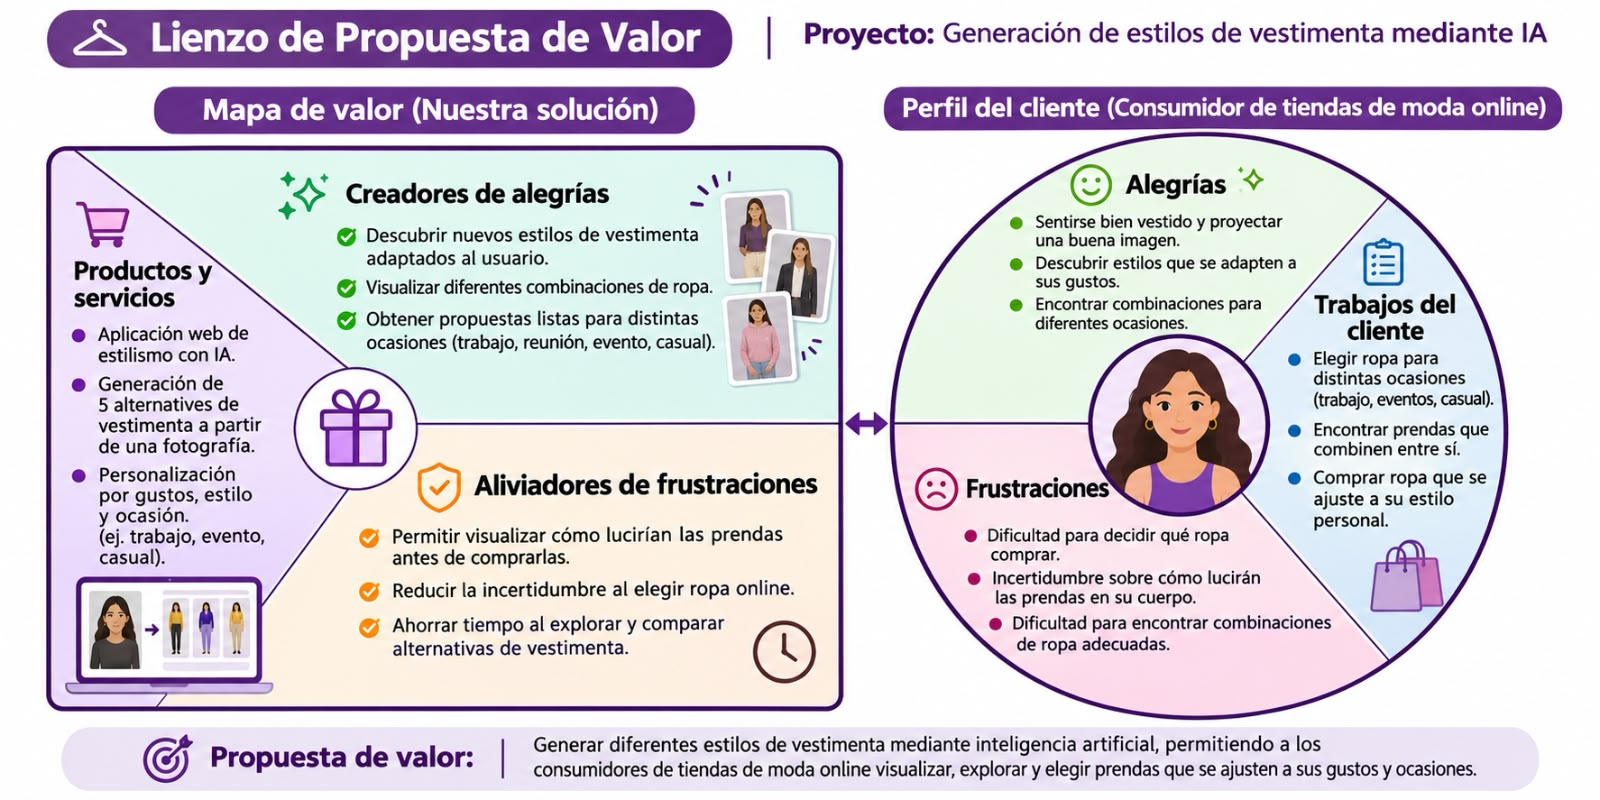
\includegraphics[width=0.86\textwidth]{figs/lienzo_valor.png}
\caption{Lienzo de propuesta de valor: perfil del consumidor de tiendas de moda en línea y mapa de valor.}
\end{figure}

\begin{table}[H]
\centering
\caption{Las tres preguntas del producto.}
\small
\begin{tabularx}{\textwidth}{@{}p{2.6cm}L@{}}
\toprule
\textbf{¿Qué es?} & Un probador virtual web con IA que, a partir de una foto del cliente, genera cinco looks según la
ocasión, las prendas del catálogo o una instrucción propia, con dos maneras de generar a elegir (una local y gratuita, y
otra por API de pago), revisión por imagen o por paquete, historial restaurable y un resumen explicado y verificado. \\
\textbf{¿Para quién es?} & Usuario final: consumidores de tiendas de moda en línea. Cliente que paga: las tiendas, que
integran el probador en su web (modelo B2B2C). \\
\textbf{¿Para qué sirve?} & Para que el consumidor compre con más confianza y descubra combinaciones por ocasión
(trabajo, reunión, evento, casual), y para que la tienda conozca sus preferencias a partir de un registro explícito de
aceptadas y rechazadas. \\
\bottomrule
\end{tabularx}
\end{table}

\textbf{Design thinking.} Empatizar, definir el punto de vista \emph{``necesito saber cómo me queda una prenda y con
qué combinarla antes de pagar''}, idear, prototipar y testear. Las entrevistas con compradores y las pruebas con
participantes \textbf{aún no se realizaron}; no reportamos cifras de mercado ni de ventas, y los supuestos de negocio
se marcan como tales (Sección~\ref{sec:eval}).

% ------------------------------------------------------------------ 3
\section{Objetivos y requisitos}

\textbf{Objetivo general.} Desarrollar un probador virtual generativo que muestre al cliente cinco looks sobre su
propia foto, controlados por sus decisiones y explicados por un agente LLM fiel a ellas. La Tabla~\ref{tab:oe} resume
el estado de cada objetivo específico.

\begin{table}[H]
\centering
\caption{Objetivos específicos (un verbo cada uno) y su estado al cierre.}
\label{tab:oe}
\small
\begin{tabularx}{\textwidth}{@{}p{0.9cm}p{5.6cm}L@{}}
\toprule
\textbf{OE} & \textbf{Objetivo} & \textbf{Estado y evidencia} \\
\midrule
OE1 & Diseñar la arquitectura y la experiencia de usuario & Cumplido: Sección~\ref{sec:diseno} y interfaz propia \\
OE2 & Preparar las fotos y el catálogo para la generación & Parcial: fotos de prueba y catálogo curado; sin dataset propio con consentimiento \\
OE3 & Implementar dos maneras de generar cinco looks por foto & Cumplido: intermedio local y básico por API (Sección~\ref{sec:impl}) \\
OE4 & Desarrollar una interfaz que registre decisiones e itere & Cumplido: nueva ronda, historial y restauración \\
OE5 & Integrar un agente LLM verificado contra el registro & Cumplido con 2 LLM y verificador determinista \\
OE6 & Incorporar guardrails de entrada y de salida & Cumplido (Sección~\ref{sec:etica}) \\
OE7 & Evaluar con métricas de generación, explicabilidad, uso y negocio & Parcial: sin pruebas con participantes (Sección~\ref{sec:eval}) \\
\bottomrule
\end{tabularx}
\end{table}

\begin{table}[H]
\centering
\caption{Requisitos funcionales (RF) y restricciones (R).}
\small
\begin{tabularx}{\textwidth}{@{}p{0.75cm}L|p{0.6cm}L@{}}
\toprule
\multicolumn{2}{@{}l|}{\textbf{Requisitos funcionales}} & \multicolumn{2}{l@{}}{\textbf{Restricciones}} \\
\midrule
RF1 & Cargar y validar una foto del cliente. & R1 & Equipo local: GPU de 4 GB y 15,7 GB de RAM; Colab y Kaggle gratuitos con cuota limitada. \\
RF2 & Elegir la manera de generar y una ocasión, prendas o una instrucción. & R2 & Gratuito por defecto: la API es opcional, de pago y con consentimiento. \\
RF3 & Generar exactamente cinco looks (V1--V5). & R3 & Solo modelos con licencia compatible con el uso. \\
RF4 & Aceptar o rechazar cada look, o el paquete. & R4 & Solo fotos con consentimiento; no se publican fotos de terceros. \\
RF5 & Regenerar solo los rechazados. & R5 & Plazo del curso y equipo de cinco personas. \\
RF6 & Guardar historial y restaurar una ronda. & R6 & Video $\le$ 3 min y demo en vivo $\le$ 6 min. \\
RF7 & Resumir con uno de dos LLM y verificar. & R7 & Informe de 10 páginas como máximo. \\
RF8 & Guardar los looks aceptados y ver métricas. & & \\
\bottomrule
\end{tabularx}
\end{table}

% ------------------------------------------------------------------ 4
\section{Vigilancia tecnológica y selección de modelos}

Revisamos modelos abiertos en Hugging Face y servicios comerciales. La Tabla~\ref{tab:modelos} indica qué usamos, qué
probamos y qué dejamos como trabajo futuro; las licencias son las declaradas en cada ficha y no constituyen una
verificación legal.

\begin{table}[H]
\centering
\caption{Modelos evaluados y su estado.}
\label{tab:modelos}
\small
\begin{tabularx}{\textwidth}{@{}p{3.9cm}p{2.2cm}L@{}}
\toprule
\textbf{Modelo} & \textbf{Estado} & \textbf{Rol y licencia} \\
\midrule
SD 1.5 Inpainting & Usado & Regenera solo la zona de la ropa (intermedio); CreativeML OpenRAIL-M \\
ControlNet 1.1 OpenPose & Usado & Mantiene la pose del cliente; OpenRAIL \\
SegFormer B2 (ATR) & Usado & Máscaras de ropa, rostro y cabello; licencia por verificar \\
ViTPose base & Usado & Ubica muñecas y manos; Apache-2.0 \\
CLIP ViT-B/32 & Usado & Elige entre candidatos y mide $\Delta$CLIP; MIT (código) \\
gpt-image-2 (OpenAI, API) & Usado & Básico por API; de pago, términos del servicio \\
SD 1.5 + LoRA propio & Entrenado, no adoptado & Experimento del nivel avanzado (Sección~\ref{sec:lora}) \\
Qwen2.5-1.5B, Phi-3.5-mini & Usados & Los dos LLM que explican; Apache-2.0 y MIT \\
IP-Adapter, IDM-VTON & No probados & Prenda exacta a partir de su foto; trabajo futuro \\
\bottomrule
\end{tabularx}
\end{table}

\textbf{Decisión.} Elegimos dos de los tres niveles del enunciado. El \textbf{básico} usa un servicio comercial
(API de imágenes), que es la forma más fiel en colores pero de pago, sin semilla fija y con la foto fuera del equipo. El
\textbf{intermedio} corre en local, es gratuito y reproducible, y conserva el rostro por construcción porque solo
regenera la ropa. El cliente elige cuál usar y, si uno falla, queda el otro. Exploramos además el \textbf{avanzado}
(un LoRA propio), que no se adoptó. Las prendas son \emph{descripciones} y no artículos concretos: reproducir una prenda
exacta exige que la tienda aporte sus fotos (Sección~\ref{sec:fin}).

% ------------------------------------------------------------------ 5
\section{Diseño del sistema}
\label{sec:diseno}

\begin{figure}[H]
\centering
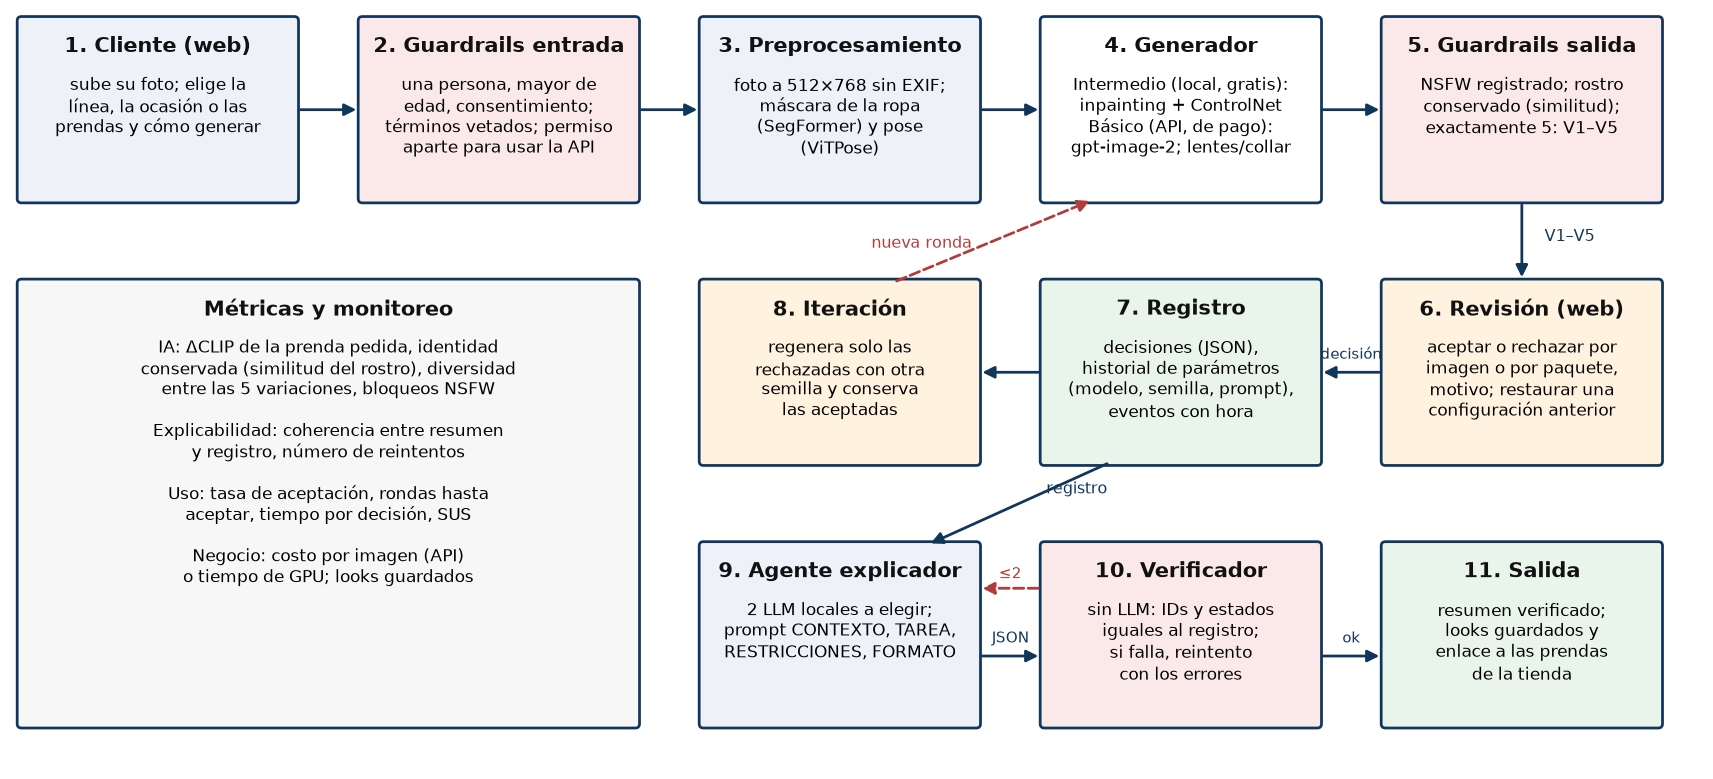
\includegraphics[width=\textwidth]{figs/arquitectura.png}
\caption{Arquitectura y flujo de información y decisiones. Las flechas rojas discontinuas son ciclos de corrección:
nueva ronda sobre los looks rechazados y reintento del LLM con los errores del verificador.}
\end{figure}

La aplicación es una sola interfaz web (Gradio) que se ejecuta en la laptop del equipo, sin notebook; el mismo código
corre en Colab o Kaggle como respaldo. \textbf{Ocasiones y catálogo.} Cuatro ocasiones (\emph{Trabajo}, \emph{Reunión},
\emph{Evento} y \emph{Casual}) y dos líneas (mujer y hombre) definen listas de looks; los looks de hombre son conjuntos
completos con pantalón y solo \emph{Casual} admite short. \textbf{Semillas e historial.} En modo prueba la semilla es
fija (1001 más 100 por ronda más la posición del look), de modo que la misma entrada reproduce las mismas imágenes; en
producción se sortea. Cada ronda guarda en el historial el enfoque, el modelo, las semillas y los textos, y permite
restaurarla. \textbf{Explicación.} El agente recibe el registro, redacta el resumen y un verificador determinista
compara identificadores y estados; si falla reintenta hasta dos veces; si sigue fallando, el programa fija el estado de cada look y el LLM solo reescribe el motivo (las listas de aceptadas y rechazadas salen siempre del registro) y, como último recurso, usa una plantilla marcada como tal.

% ------------------------------------------------------------------ 6
\section{Implementación}
\label{sec:impl}

\subsection{Intermedio: inpainting local de la ropa}
SegFormer segmenta ropa, piel, rostro y cabello, y ViTPose ubica las muñecas. La máscara cubre la prenda y, si es de
manga larga, también los brazos; \textbf{las manos se protegen} (círculo más allá de la muñeca, solo píxeles de piel) y del
cabello solo se protege el núcleo para que la tela pase bajo el borde. La zona se amplía a 640 px, se regenera con SD 1.5
Inpainting y ControlNet de pose (20 pasos, Euler) y se pega de vuelta; se generan dos candidatos por look y CLIP elige el
más cercano al texto, penalizando los estampados que el modelo inventa. Cada descripción lleva un solo color por
prenda. Después se limpia el fondo junto a la silueta. Los \textbf{accesorios} (lentes y collar) se pintan en una segunda
pasada sobre una zona pequeña ubicada con la pose; el collar solo se dibuja sobre piel visible.

\subsection{Básico: API de imágenes}
El enfoque envía la foto a la API de OpenAI (\texttt{gpt-image-2}) con la descripción del look y la instrucción de
conservar rostro, manos, zapatos, pose y fondo; los accesorios van en la misma llamada. Tras recibir la imagen se
devuelven el rostro y el núcleo del cabello de la foto original. Exige una casilla de consentimiento aparte, registra
las imágenes y el costo estimado, y no admite semilla fija.

\subsection{Catálogo curado con modelos reales}
El catálogo final tiene 33 prendas (8 de mujer y 25 de hombre) y 8 accesorios. Cada prenda se probó con los modelos
reales sobre fotos de prueba; \textbf{retiramos alrededor de 25} por fallas repetidas (colores mezclados, mangas o manos
defectuosas) y descartamos el calzado y los aretes porque salían deformados. Con pantalón en la foto no se ofrecen
vestidos ni shorts, porque el modelo no logra dibujar las piernas.

\subsection{Interfaz}
La identidad visual es \textbf{la cinta métrica}: una cinta amarilla con las marcas 1 a 5 recorre la cabecera y cada look
cuelga de su propio tramo, que se marca al decidir («Aceptado» o «Descartado», con la foto atenuada y tachada). Las dos
maneras de generar se ven siempre; el modelo que explica y el modo prueba quedan en ajustes avanzados. La Figura~\ref{fig:ui}
muestra el estado inicial. Una revisión heurística con la lista de Nielsen (autoevaluación asistida por IA) dio 24/40
antes de corregir los cuatro problemas mayores; no sustituye las pruebas con usuarios.

\begin{figure}[H]
\centering
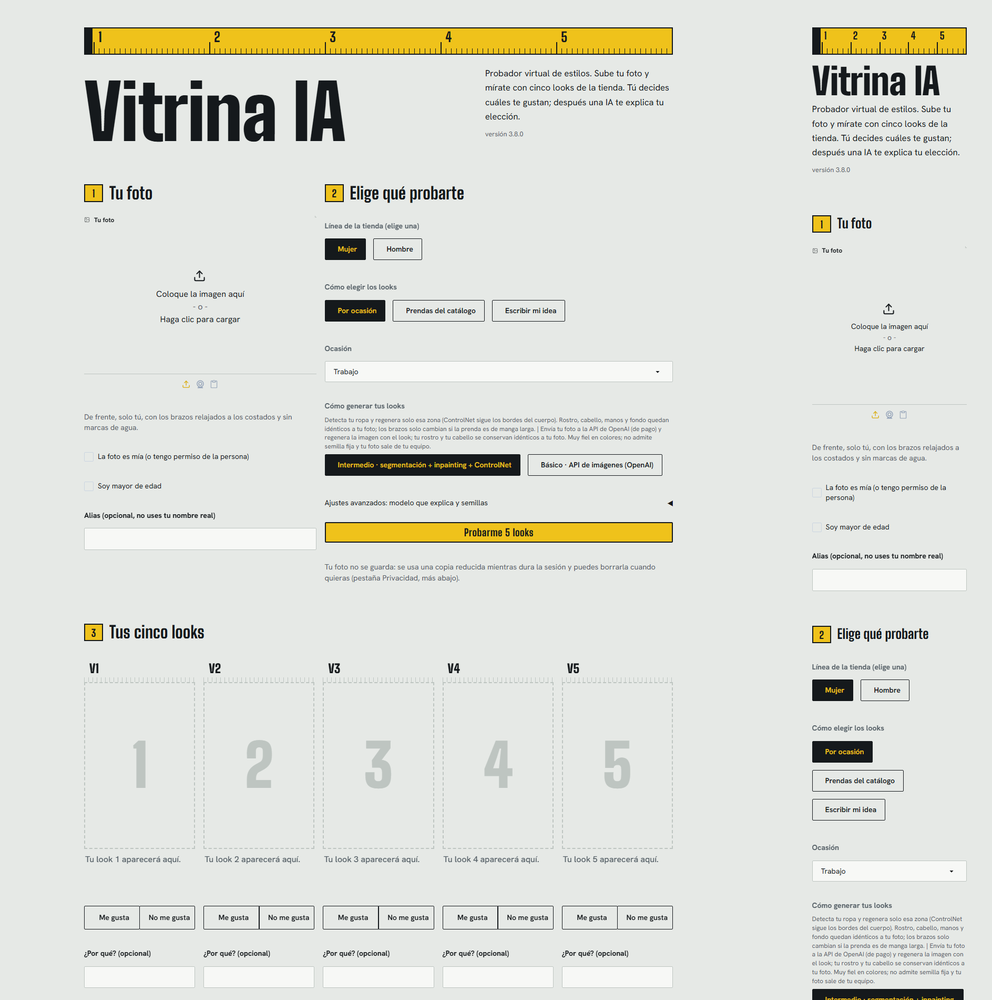
\includegraphics[height=9.4cm]{figs/interfaz.png}\hfill
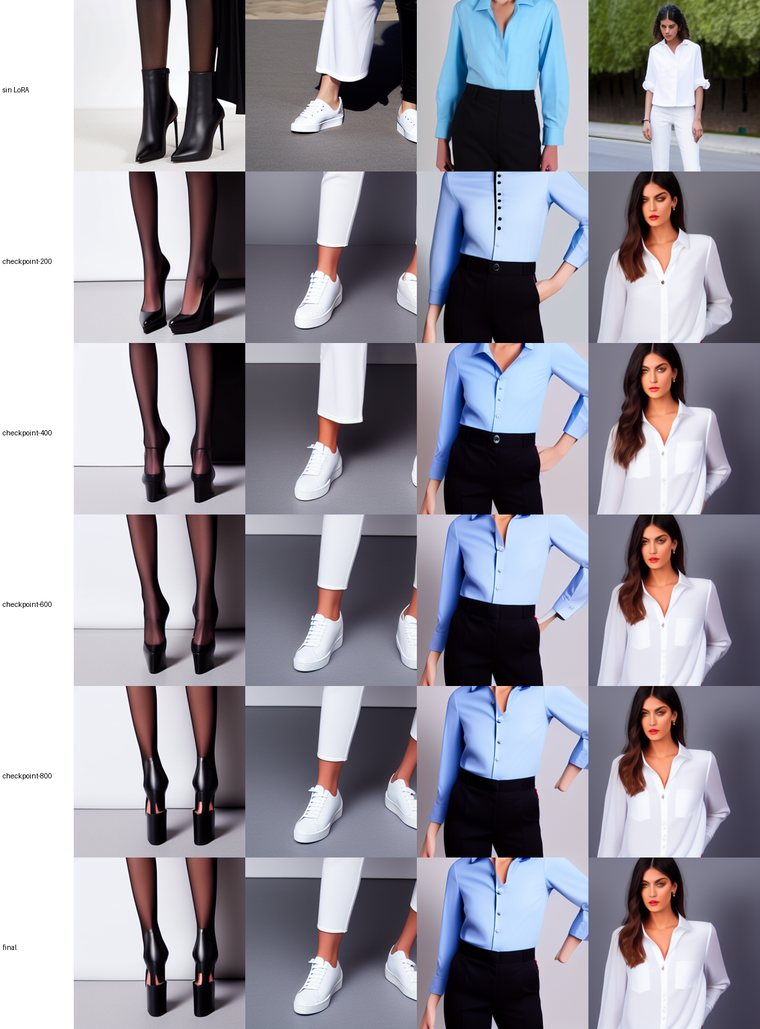
\includegraphics[height=9.4cm]{figs/lora_comparacion.jpg}
\caption{Izquierda: interfaz en escritorio y móvil (estado inicial; el recuadro «Aceptado/Descartado» aparece al decidir).
Derecha: comparación del LoRA (Sección~\ref{sec:lora}); filas: sin LoRA y puntos de control a los 200, 400, 600 y 800
pasos y el final; columnas: tacones, zapatillas, camisa celeste y blusa blanca. Todas las personas son sintéticas.}
\label{fig:ui}
\end{figure}

% ------------------------------------------------------------------ 7
\section{Nivel avanzado: un LoRA propio como experimento}
\label{sec:lora}

\textbf{Qué se hizo.} Por indicación de la profesora, entrenamos un LoRA [6] sobre SD 1.5 para que el probador
reprodujera mejor prendas concretas. Los datos son un \textbf{catálogo sintético} generado con SD 1.5 (los datasets abiertos
de ropa tienen fotos sueltas y desordenadas, poco parecidas a un catálogo): 29 prendas definidas y, en el piloto, cuatro
(tacones negros, zapatillas blancas, camisa celeste y blusa blanca) con 120 imágenes, de las que \textbf{curamos 76}. En
la primera tanda detectamos que el color se contaminaba (una blusa «blanca» con pantalón gris salía gris) y que el calzado
salía en poses imposibles, por lo que corregimos los textos y añadimos fotos de producto del calzado. El entrenamiento
corrió en Colab (T4): solo el UNet, rango 16, 800 pasos, tasa 1e-4, guardando cada 200 pasos; el archivo pesa 12,8 MB.

\textbf{Resultados.} (i) A partir de los 400 pasos el calzado se deforma (tacones con bloques y agujeros) y a los 800
aparecen artefactos en las camisas: el sobreajuste con 76 imágenes es real; el mejor punto fue el de 200. (ii) Aparece una
\textbf{fuga de identidad}: todas las blusas muestran la misma mujer del entrenamiento. (iii) Aplicado al probador (por
inpainting, misma foto y mismas semillas, cinco looks), el LoRA solo mejoró uno y empeoró o igualó el resto (camisas más
saturadas, un jean que salió blanco), por lo que \textbf{no se adoptó}. El análisis pedido para este nivel (retos de
entrenamiento, control y estabilidad) queda documentado con estos resultados; el hardware de la universidad (A100 y
A6000 por fracciones) sí alcanzaría, pero su cola de trabajos largos no era confiable para el plazo.

% ------------------------------------------------------------------ 8
\section{Guardrails y consideraciones éticas}
\label{sec:etica}

\begin{table}[H]
\centering
\caption{Guardrails implementados y riesgo que mitigan.}
\small
\begin{tabularx}{\textwidth}{@{}p{3.1cm}Lp{3.3cm}@{}}
\toprule
\textbf{Guardrail} & \textbf{Funcionamiento} & \textbf{Riesgo} \\
\midrule
Consentimiento y edad & Declaración de que la foto es suya y de que es mayor de edad; máximo una persona & Fotos de terceros o menores \\
Consentimiento de la API & Casilla aparte antes de enviar la foto a OpenAI; sin ella no se envía nada & Foto fuera del equipo \\
Prendas y términos & Lista cerrada de prendas y términos vetados (también en la traducción) & Sexualización, marcas \\
Cuerpo y rostro & La máscara cubre solo la ropa; se compara el rostro con el original (umbral 0,45) & Cambios de identidad \\
Filtro NSFW & Safety checker sobre cada imagen generada; solo se registra (ver abajo) & Contenido sexual \\
Privacidad & No se guarda la foto; copia reducida solo durante la sesión; botón para borrarla & Datos biométricos \\
Etiquetado y verificador & Etiqueta «Simulación IA»; verificación del resumen con plantilla de respaldo & Engaño, alucinación \\
\bottomrule
\end{tabularx}
\end{table}

\textbf{Reflexión.} El mayor riesgo es la \textbf{sexualización y los \emph{deepfakes}}: un sistema que «cambia la ropa» puede
usarse para desvestir. Lo mitigamos de forma preventiva (lista cerrada, máscara limitada a la ropa, términos vetados) y
no solo con un filtro posterior. De hecho, el filtro NSFW de SD dio \textbf{falsos positivos con ropa normal} (suéteres,
blazers) y nos hizo mostrar imágenes negras; por eso decidimos \textbf{registrarlo y no bloquear}, a costa de depender de
la prevención. También hay \textbf{sesgos}: los modelos de difusión representan mejor ciertos cuerpos y tonos, y los
datos sintéticos heredan los sesgos del generador (la fuga de identidad del LoRA lo ilustra). Con la API la foto sale
del equipo, de ahí el consentimiento aparte. Por último, la foto es un dato personal (Ley N.º 29733) y la simulación debe
presentarse como tal (Ley N.º 29571). \textbf{No se publican fotos de terceros} en este repositorio.

% ------------------------------------------------------------------ 9
\section{Evaluación}
\label{sec:eval}

\begin{table}[H]
\centering
\caption{Resultados medidos. Las muestras son pequeñas (una foto de prueba y cinco looks por conjunto): son exploratorios.}
\small
\begin{tabularx}{\textwidth}{@{}p{3.2cm}Lp{3.0cm}@{}}
\toprule
\textbf{Dimensión} & \textbf{Resultado} & \textbf{Límite} \\
\midrule
Cinco looks por solicitud & Siempre 5; comprobado por las pruebas automáticas & Con modelos simulados \\
Coherencia del resumen & Un verificador sin LLM comprueba cada resumen; en el piloto previo el LLM acertó solo en 3 de 4 sesiones y ningún resumen incoherente llegó al usuario & Pruebas y piloto previo \\
Colores correctos & API: 5 de 5 looks; intermedio: 3 de 5 (pantalón «negro» azul, blusa «blanca» negra) & Una foto, revisión visual \\
Identidad & Intermedio: rostro fuera de la máscara. API: SSIM de la caja del rostro de 0,74 a 0,80 tras restaurar rostro y cabello & La caja incluye cuello y cuello de la prenda \\
Tiempo por 5 looks & API: unos 130 s; intermedio: de 2 a 5 min en la GPU de 4 GB (de 40 a 60 s en versiones sin accesorios) & Depende de la memoria libre \\
Costo & API: unos \$0{,}023 por imagen (el saldo bajó de \$10{,}00 a \$9{,}86 tras 6 imágenes), unos \$0{,}12 por prueba; local: \$0 & Estimado y redondeado \\
Avanzado (LoRA) & Sin mejora neta; sobreajuste desde los 400 pasos; fuga de identidad & Un piloto de 4 prendas \\
Usabilidad (SUS) & Cuestionario implementado en la app; \textbf{sin participantes aún} & Pendiente \\
\bottomrule
\end{tabularx}
\end{table}

\textbf{Viabilidad y negocio.} El costo variable de la API es de centavos por prueba, y el del enfoque local es cero pero
más lento y limitado por la memoria. El modelo B2B2C propuesto (la tienda paga por pruebas) y su precio, el efecto sobre
ventas o devoluciones y la disposición a pagar son \textbf{supuestos a validar}, no resultados.

% ------------------------------------------------------------------ 10
\section{Limitaciones y trabajo pendiente}
\label{sec:fin}

\begin{itemize}
\item \textbf{Colores mezclados en el intermedio.} Con dos prendas de distinto color en una frase, SD 1.5 las mezcla o las
intercambia. La solución pensada es pintar arriba y abajo en dos pasadas con una prenda cada una; no está aplicada.
\item \textbf{Prendas descritas, no exactas.} Para reproducir un artículo concreto la tienda debe aportar fotos de sus
prendas y usar un método con imagen de referencia (IP-Adapter u otro), que no probamos.
\item \textbf{Falta de pruebas con usuarios.} No hay aún cuestionario SUS con participantes ni el video con un participante
externo; ambos son parte de la entrega.
\item \textbf{Poses y fotos difíciles.} Manos sobre el cuello o ropa muy holgada fallan; pedimos foto frontal con brazos
relajados. El calzado y los aretes quedaron fuera por no salir bien.
\item \textbf{Memoria.} En la laptop de 4 GB, el intermedio compite por la memoria con otros programas.
\end{itemize}

\begin{table}[H]
\centering
\caption{Cumplimiento de los requisitos del enunciado.}
\small
\begin{tabularx}{\textwidth}{@{}p{5.2cm}p{2.0cm}L@{}}
\toprule
\textbf{Requisito} & \textbf{Estado} & \textbf{Evidencia o pendiente} \\
\midrule
Exactamente cinco variaciones por foto & Cumplido & Pruebas automáticas y sesiones reales \\
Interfaz para aceptar o rechazar cada una & Cumplido & Por imagen o por paquete, con motivo opcional \\
Decisiones registradas de forma estructurada & Cumplido & Registro de decisiones, eventos e historial \\
Agente LLM coherente con el registro & Cumplido & Dos LLM y verificador determinista \\
Dos de tres niveles de implementación & Cumplido & Básico (API) e intermedio; avanzado explorado \\
Guardrails; semilla fija y variable; historial & Cumplido & Sección~\ref{sec:etica} y Sección~\ref{sec:diseno} \\
Vigilancia tecnológica de modelos & Cumplido & Tabla~\ref{tab:modelos} \\
Dataset justificado y análisis exploratorio & Parcial & Fotos de prueba y catálogo curado; sin dataset propio \\
Métricas de calidad, diversidad, coherencia y usabilidad & Parcial & Falta el SUS con participantes \\
Reflexión ética & Cumplido & Sección~\ref{sec:etica} \\
Video (3 min) con un participante externo & Pendiente & Guion listo; falta grabarlo \\
Demostración en vivo (6 min) & Pendiente & Guion listo \\
Informe de 10 páginas como máximo & Cumplido & 9 páginas, compilado con pdfLaTeX \\
\bottomrule
\end{tabularx}
\end{table}

% ------------------------------------------------------------------ referencias
\section*{Referencias}
\footnotesize
\begin{enumerate}[label={[\arabic*]},leftmargin=2.2em,itemsep=0pt]
\item R. Rombach et al., ``High-Resolution Image Synthesis with Latent Diffusion Models'', CVPR, 2022.
\item L. Zhang, A. Rao y M. Agrawala, ``Adding Conditional Control to Text-to-Image Diffusion Models'', ICCV, 2023.
\item Z. Cao et al., ``OpenPose: Realtime Multi-Person 2D Pose Estimation Using Part Affinity Fields'', IEEE TPAMI, 2021.
\item E. Xie et al., ``SegFormer: Simple and Efficient Design for Semantic Segmentation with Transformers'', NeurIPS, 2021.
\item Y. Xu et al., ``ViTPose: Simple Vision Transformer Baselines for Human Pose Estimation'', NeurIPS, 2022.
\item E. J. Hu et al., ``LoRA: Low-Rank Adaptation of Large Language Models'', ICLR, 2022 (arXiv:2106.09685).
\item A. Radford et al., ``Learning Transferable Visual Models From Natural Language Supervision'', ICML, 2021.
\item Qwen Team, ``Qwen2.5 Technical Report'', arXiv:2412.15115, 2024.
\item M. Abdin et al., ``Phi-3 Technical Report'', arXiv:2404.14219, 2024.
\item H. Ye et al., ``IP-Adapter: Text Compatible Image Prompt Adapter for Text-to-Image Diffusion Models'', arXiv:2308.06721, 2023.
\item Y. Choi et al., ``Improving Diffusion Models for Authentic Virtual Try-on in the Wild'' (IDM-VTON), ECCV, 2024.
\item J. Brooke, ``SUS: A Quick and Dirty Usability Scale'', en \emph{Usability Evaluation in Industry}, 1996.
\item J. Nielsen, ``10 Usability Heuristics for User Interface Design'', Nielsen Norman Group, 1994.
\item Congreso de la República del Perú, Ley N.º 29733, Ley de Protección de Datos Personales, 2011.
\item Congreso de la República del Perú, Ley N.º 29571, Código de Protección y Defensa del Consumidor, 2010.
\end{enumerate}

\end{document}
